\documentclass[a4paper,12pt]{extarticle}
\usepackage[utf8x]{inputenc}
\usepackage[T1,T2A]{fontenc}
\usepackage[russian]{babel}
\usepackage{hyperref}
\usepackage{indentfirst}
\usepackage{listings}
\usepackage{color}
\usepackage{here}
\usepackage{array}
\usepackage{multirow}
\usepackage{graphicx}
\usepackage{amsmath}
\usepackage{amssymb}
\usepackage{makeidx}    

\usepackage{caption}
\renewcommand{\lstlistingname}{Программа} % заголовок листингов кода

\bibliographystyle{ugost2008ls}

\usepackage{listings}
\lstset{ %
extendedchars=\true,
keepspaces=true,
language=C,						% choose the language of the code
basicstyle=\footnotesize,		% the size of the fonts that are used for the code
numbers=left,					% where to put the line-numbers
numberstyle=\footnotesize,		% the size of the fonts that are used for the line-numbers
stepnumber=1,					% the step between two line-numbers. If it is 1 each line will be numbered
numbersep=5pt,					% how far the line-numbers are from the code
backgroundcolor=\color{white},	% choose the background color. You must add \usepackage{color}
showspaces=false				% show spaces adding particular underscores
showstringspaces=false,			% underline spaces within strings
showtabs=false,					% show tabs within strings adding particular underscores
frame=single,           		% adds a frame around the code
tabsize=2,						% sets default tabsize to 2 spaces
captionpos=t,					% sets the caption-position to top
breaklines=true,				% sets automatic line breaking
breakatwhitespace=false,		% sets if automatic breaks should only happen at whitespace
escapeinside={\%*}{*)},			% if you want to add a comment within your code
postbreak=\raisebox{0ex}[0ex][0ex]{\ensuremath{\color{red}\hookrightarrow\space}},
texcl=true,
inputpath=source,                     % директория с листингами
}

\usepackage[left=2cm,right=2cm,
top=2cm,bottom=2cm,bindingoffset=0cm]{geometry}

%% Нумерация картинок по секциям
\usepackage{chngcntr}
\counterwithin{figure}{section}
\counterwithin{table}{section}

%%Точки нумерации заголовков
\usepackage{titlesec}
\titlelabel{\thetitle.\quad}
\usepackage[dotinlabels]{titletoc}

%% Оформления подписи рисунка
\addto\captionsrussian{\renewcommand{\figurename}{Рисунок}}
\captionsetup[figure]{labelsep = period}

%% Подпись таблицы
\DeclareCaptionFormat{hfillstart}{\hfill#1#2#3\par}
\captionsetup[table]{format=hfillstart,labelsep=newline,justification=centering,skip=-10pt,textfont=bf}

%% Путь к каталогу с рисунками
\graphicspath{{pictures/}}


\begin{document}	% начало документа

% Титульная страница
\begin{titlepage}	% начало титульной страницы

	\begin{center}		% выравнивание по центру

		\large Санкт-Петербургский Политехнический Университет Петра Великого\\
		\large Институт компьютерных наук и технологий \\
		\large Кафедра компьютерных систем и программных технологий\\[6cm]
		% название института, затем отступ 6см
		
		\huge Телекоммуникационные технологии\\[0.5cm] % название работы, затем отступ 				%0,5см
		\large Отчет по лабораторной работе №3\\[0.1cm]
		\large Линейная фильтрация
		\\[5cm]

	\end{center}


	\begin{flushright} % выравнивание по правому краю
		\begin{minipage}{0.25\textwidth} % врезка в половину ширины текста
			\begin{flushleft} % выровнять её содержимое по левому краю

				\large\textbf{Работу выполнил:}\\
				\large Балсутьев В.А.\\
				\large {Группа:} 33501/4\\
				
				\large \textbf{Преподаватель:}\\
				\large Богач Н.В.

			\end{flushleft}
		\end{minipage}
	\end{flushright}
	
	\vfill % заполнить всё доступное ниже пространство

	\begin{center}
	\large Санкт-Петербург\\
	\large \the\year % вывести дату
	\end{center} % закончить выравнивание по центру

\thispagestyle{empty} % не нумеровать страницу
\end{titlepage} % конец титульной страницы

\vfill % заполнить всё доступное ниже пространство
	

% Содержание
% Содержание
\renewcommand\contentsname{\centerline{Содержание}}
\tableofcontents
\newpage



\section{Цель работы}
Изучить амплитудную модуляцию/демодуляцию сигнала.

\section{Постановка задачи}
\begin{itemize}
	\item Сгенерировать однотональный сигнал низкой частоты.
	\item Выполнить амплитудную модуляцию.
	\item Получить спектр модулированного сигнала.
	\item Выполнить модуляцию с подавлением несущей.
	\item Выполнить однополосную модуляцию.
	\item Выполнить синхронное детектирование и получить исходный однополосный сигнал.
	\item Рассчиать КПД.
\end{itemize}


\section{Теоретическая информация}
\subsection{Модуляция}
Модуляция(\href{https://ru.wikipedia.org/wiki/Модуляция}{wiki}) — процесс изменения одного или нескольких параметров высокочастотного несущего колебания по закону низкочастотного информационного сигнала (сообщения). Сущность модуляции заключается в следующем. Формируется некоторое колебание (чаще всего гармоническое), называемое несущим колебанием или просто несущей (carrier), и какой-либо из параметров этого колебания изменяется во времени пропорционально исходному сигналу. Исходный сигнал называют модулирующим (modulating signal), а результирующее колебание с изменяющимися во времени параметрами — модулированным сигналом (modulated signal). Обратный процесс — выделение модулирующего сигнала из модулированного колебания — называется демодуляцией (demodulation).
Обычнно за несущий сигнал принимается гармоническое колебание вида 
$ s(t) = A \cos(\omega_0 t + \phi_0) $, где $ А $ - амплитуда, $ \omega_0 $ - циклическая частота, $t$ - время, $ \phi_0 $ - начальная фаза. Какие параметры можно использовать для процесса модуляции - 
очевидно те, которые не являются изменяемыми аргументами(параметрами) исходного несущего колебания - амплитуда, частота, фаза. Ну и по названию существуют модуляции:

\begin{itemize}
	\item амплитудная
	\item частотная
	\item фазовая
\end{itemize}   

Частотную и фазовую модуляции часто называют угловым видом модуляции, т.к. они меняют аргумент косинуса. Так же существует так называемая квадратурная модуляция, при которой изменяются, и амплитуда, и фаза сигнала. 
В данной работе мы рассматриваем только амплитудную модуляцию.

\subsection{Амплитудная модуляция}
Как явствует из названия, при амплитудной модуляции (AM; английский термин — amplitude modulation, AM) в соответствии с модулирующим сигналом изменяется амплитуда несущего колебания:
$ u_{am}(t) =  A(t) \cos( \omega_0 t + \phi_0)$.
Однако если амплитуду A(t) просто сделать прямо пропорциональной модулирующему сигналу, возможно возникновение следующей проблемы. Как правило, модулирующий сигнал является двуполярным (знакопеременным). Экспериментально доказано, что амплитудная огибающая, которая будет выделена в процессе демодуляции, в данном случае оказывается неправильной и соответсвует модулю исходного сигнала. Поэтому при реализации АМ к модулирующему сигналу предварительно добавляют постоянную составляющую, чтобы сделать его однополярным: $ A(t) =  A_0 + ks_m(t) $.
В итоге формула амплитудной модуляции в общем виде выглядит так: 
\begin{equation}\label{eq01}
	u(t) = (1 + M U_m cos(\Omega t)) cos(\omega_0 t + \phi _0)
\end{equation}
Спектр сигнала с амплитудной модуляцией показан на рис.\ref{pic:pic001_spec_amtheor}.
На графике $\omega_0$ --- частота несущей, $\Omega$ --- частота модуляции.
\begin{figure}[H]
	\begin{center}
		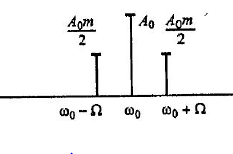
\includegraphics[scale=0.7]{spec_a_mod.png}
		\caption{Спектр амплитудно-модулированного сигнала} 
		\label{pic:pic001_spec_amtheor} % название для ссылок внутри кода
	\end{center}
\end{figure}

Амплитудная модуляция имеет низкий КПД.

\subsubsection{Амплитудная модуляция с подавлением несущей}
Основная мощность АМ сигнала приходится на несущую частоту. При АМ с подавлением несущей производится перемножение двух сигналов – модулирующего и несущего. В результате несущая частота подавляется и КПД модуляции становится 100\%.
Формула такой модуляции:
\begin{equation}\label{eq02}
	u(t) = M U_m cos(\Omega t) cos(\omega_0 t + \phi _0)
\end{equation}

Спектр сигнала с амплитудной модуляцией с подавлением несущей отличается от спектра модуляции без подавления несущей только наличием основной (несущей гармоники), которая и определяет потери в энергии. 

\subsubsection{Однополосная модуляция}
Рассмотренная в предыдущем разделе двухполосная AM с подавленной несущей имеет преимущества перед обычной AM только в энергетическом смысле — за счет устранения несущего колебания. Ширина же спектра при этом остается равной удвоенной частоте модулирующего сигнала.
Однако можно легко заметить, что спектры двух боковых полос АМ-сигнала являются зеркальным отражением друг друга, то есть они несут одну и ту же информацию. Поэтому одну из боковых полос можно удалить. Получающаяся модуляция называется однополосной (английский термин — single side band, SSB).
В зависимости от того, какая боковая полоса сохраняется, говорят ободнополосной модуляции с использованием верхней или нижней боковой полосы. Формирование однополосного сигнала проще всего пояснить, приведя несколько спектральных графиков:  

\begin{figure}[H]
	\begin{center}
		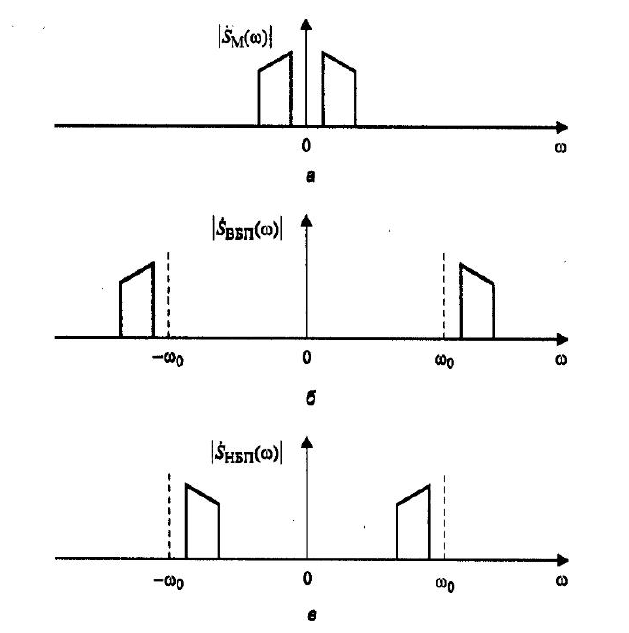
\includegraphics[scale=0.7]{spec_one_stripe.png}
		\caption{Однополосная модуляция: а - спектр модулирующего сигнала,
		б - спектр однополсоного сигнала с верхней боковой полосой, в - то же с нижней боковой 			        полосой} 
		\label{pic:spec_one_stripe} % название для ссылок внутри кода
	\end{center}
\end{figure}

По сути дела, при однополосной модуляции происходит просто сдвиг спектра сигнала в окрестности частоты несущего колебания. В отличие от AM каждая «половинка» спектра смещается в своем направлении: область положительных частот — к $ \omega_0 $, а область отрицательных частот — к $  - \omega_0 $
Очевидно, что ширина спектра однополоcного сигнала равна ширине спектра модулирующего сигнала. Таким образом, спектр однополосного сигнала оказывается в два раза уже, чем при обычной АМ.

\subsubsection{Демодуляция с помощью синхронного детектирования}
При синхронном детектировании модулированный сигнал умножается на опорное колебание с частотой несущего колебания:
 \begin{equation}\label{eq04}
 	y(t) = U(t) cos(\omega_0 t) cos(\omega_0 t) = \frac{U(t)}{2} (1 + cos(2\omega_0 t))
\end{equation}
Сигнал разделяется на два слагаемых, первое из которых повторяет исходный модулирующий сигнал, а второе повторяет модулированный сигнал на удвоенной несущей частоте 2$\omega_0$. 

Амплитудный спектр сигналов после демодуляции однозначно соотносится со спектром входного модулированного сигнала: 
амплитуды гармоник модулированного сигнала на частоте 2$\omega_0$ в два раза меньше амплитуд входного сигнала,
 постоянная составляющая равна амплитуде несущей частоты $\omega_0$ и не зависит от глубины модуляции, амплитуда
  информационного демодулированного сигнала в два раза меньше амплитуды исходного модулирующего сигнала. 

Особенностью синхронного детектирования является независимость от глубины модуляции,
 т.е. коэффициент модуляции сигнала может быть больше единицы. 
 При синхронном детектировании требуется точное совпадение фаз и частот 
 опорного колебания демодулятора и несущей гармоники АМ сигнала.

\subsubsection{КПД модуляции}
КПД амплитудной модуляции зависит от коэффициента модуляции и может быть рассчитано по следующей формуле:
 \begin{equation}\label{eq05}
	\eta (t) =\frac{ U_m^2(t) M^2}{4 P_U}  = \frac{M^2}{2 + M^2} 
\end{equation}


\section{Ход работы}

\subsection{Модуляция однотонального сигнала}
Зададим параметры несущего колебания и модулируемого однотонального сигнала.
С помощью функций встроенного пакета Communications, проведем амплитудную модуляцию и построим спектры. Данную последовательность операций повторим для разных значений параметра m - коэффицента модуляции.

\begin{figure}[H]
	\begin{center}
		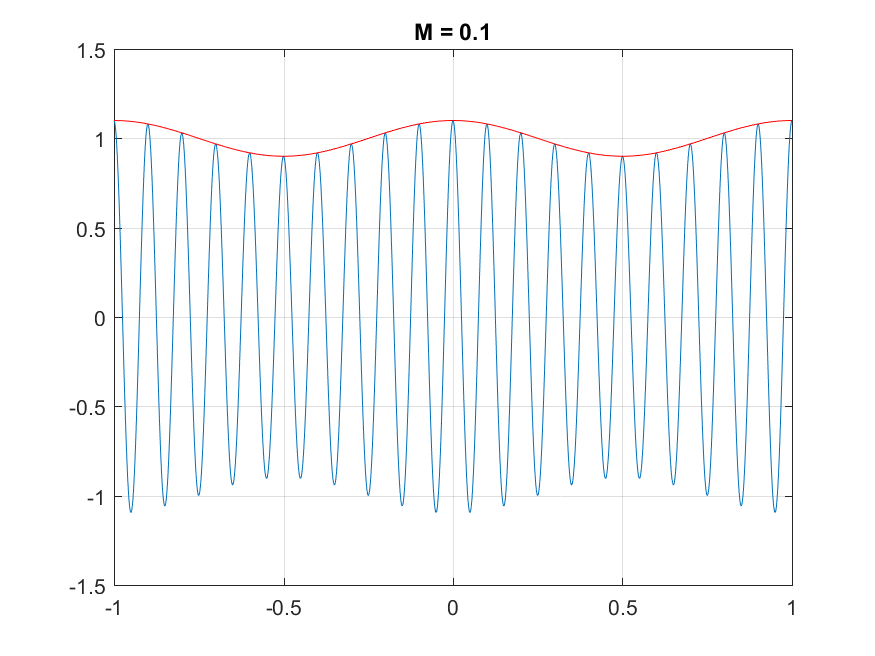
\includegraphics[scale=0.7]{sigm01.png}
		\caption{Результат АМ для m = 0.1} 
		\label{pic:pic01} % название для ссылок внутри кода
	\end{center}
\end{figure} 
При данном коэффициенте модуляции, очевидно, что амплитудная модуляция не соотвествует однотональному сигналу.  
\begin{figure}[H]
	\begin{center}
		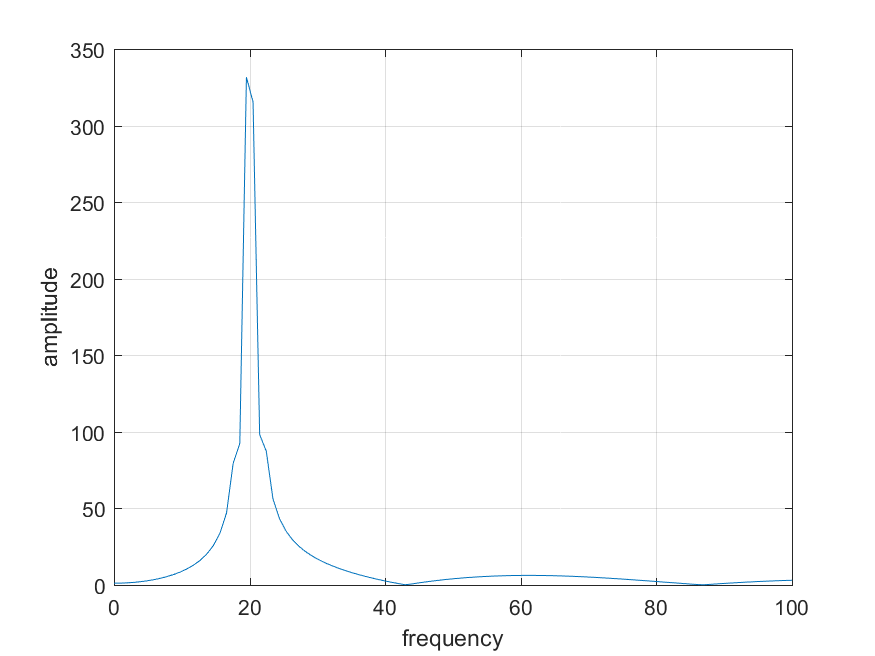
\includegraphics[scale=0.7]{specm01.png}
		\caption{Амплитудный спектр для m = 0.1} 
		\label{pic:pic02} % название для ссылок внутри кода
	\end{center}
\end{figure} 
%%%%%%%%%%%%%%%%%%%%%%%%%%%%%%%%%%%%%%%%%%%%%%%%%%%%%%%%

Положив m = 0.6, получаем достаточно неплохую модуляцию. 
\begin{figure}[H]
	\begin{center}
		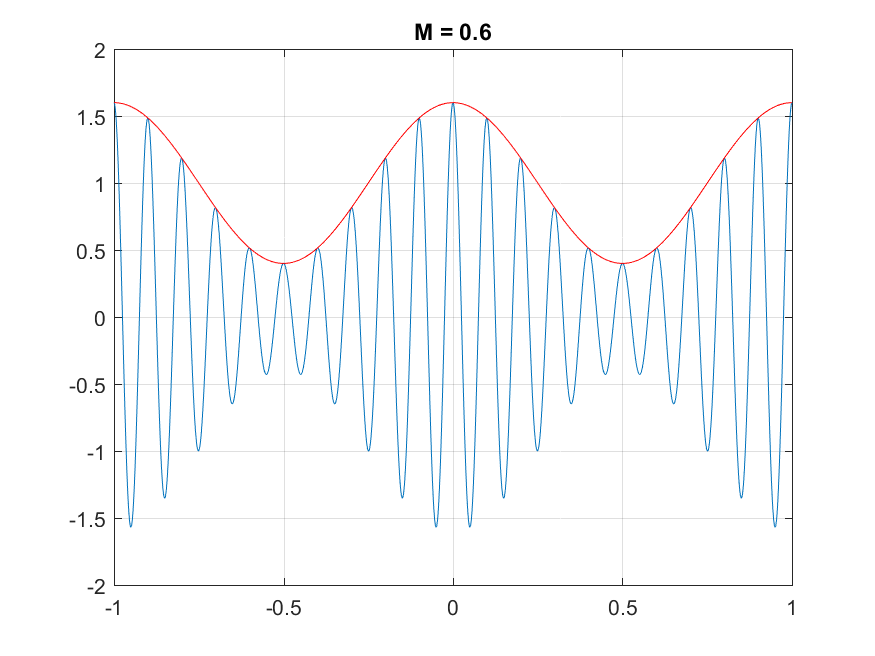
\includegraphics[scale=0.7]{sigm06.png}
		\caption{Результат АМ для m = 0.6} 
		\label{pic:pic01} % название для ссылок внутри кода
	\end{center}
\end{figure} 
Также на спектре явно видна несущая гармоника и 2 информационные гармоники.
\begin{figure}[H]
	\begin{center}
		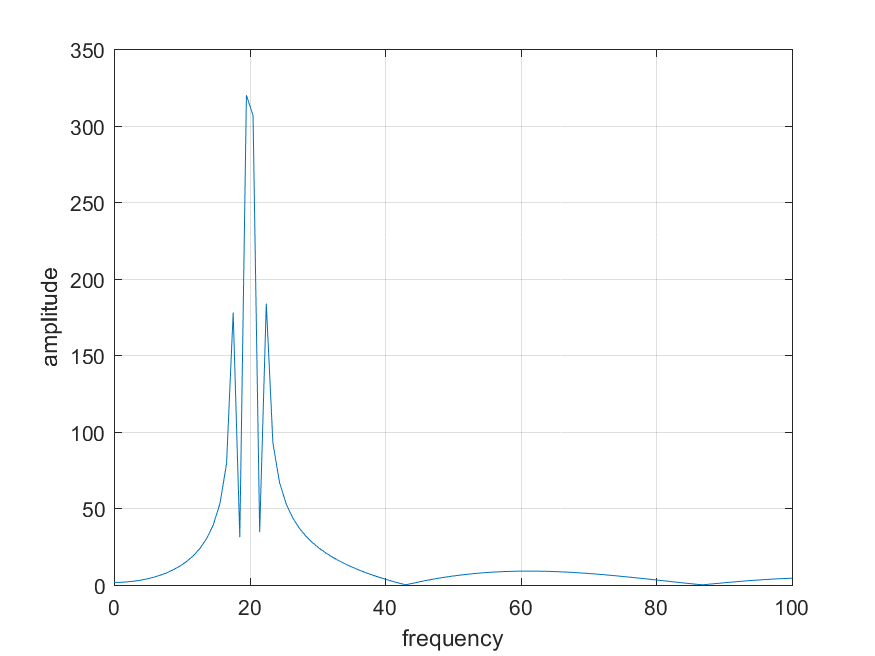
\includegraphics[scale=0.7]{specm06.png}
		\caption{Амплитудный спектр для m = 0.6} 
		\label{pic:pic02} % название для ссылок внутри кода
	\end{center}
\end{figure} 
%%%%%%%%%%%%%%%%%%%%%%%%%%%%%%%%%%%%%%%%%%%%%%%%%%%%%%%%
Положив m = 1.1, получаем модуляцию, соответсвтующей однотональному сигналу,
но вместе с этим небольшая перемодуляция которую можно обнаружить в минимуме нашей амплитудной огибающей. 
\begin{figure}[H]
	\begin{center}
		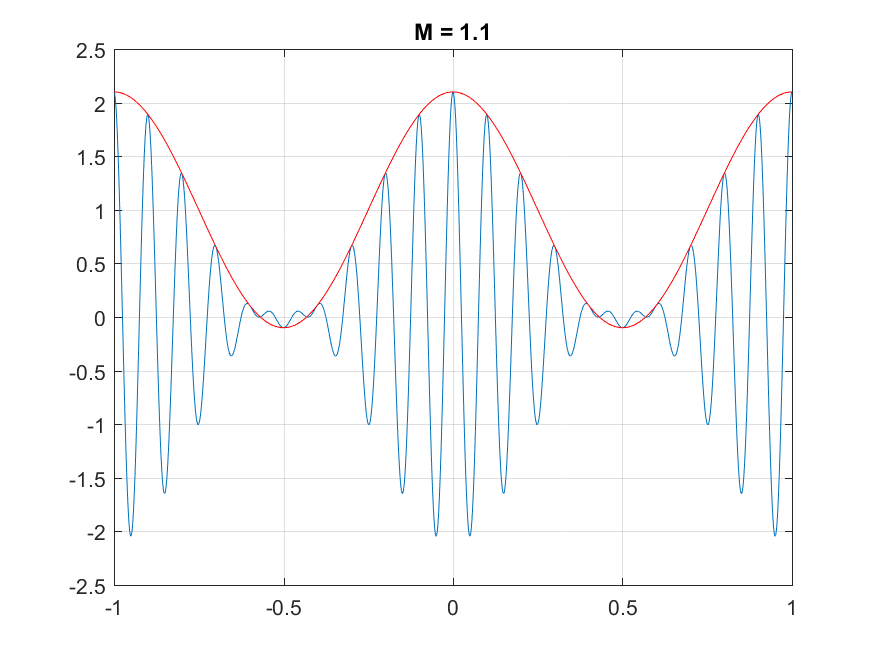
\includegraphics[scale=0.7]{sigm11.png}
		\caption{Результат АМ для m = 1.1} 
		\label{pic:pic01} % название для ссылок внутри кода
	\end{center}
\end{figure} 

\begin{figure}[H]
	\begin{center}
		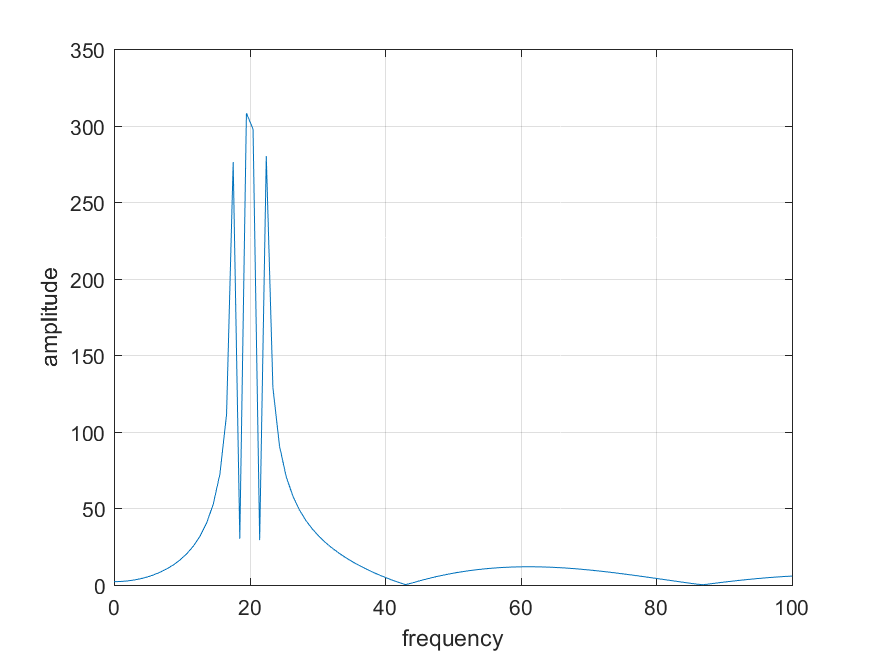
\includegraphics[scale=0.7]{specm11.png}
		\caption{Амплитудный спектр для m = 1.1} 
		\label{pic:pic02} % название для ссылок внутри кода
	\end{center}
\end{figure}
%%%%%%%%%%%%%%%%%%%%%%%%%%%%%%%%%%%%%%%%%%%%%%%%%%%%%%%%%%%
Далее при увелечении коэффициента модуляции, прекрасно видно явление перемодуляции,\
причем как по огибающей, так и по спектрам.  
\begin{figure}[H]
	\begin{center}
		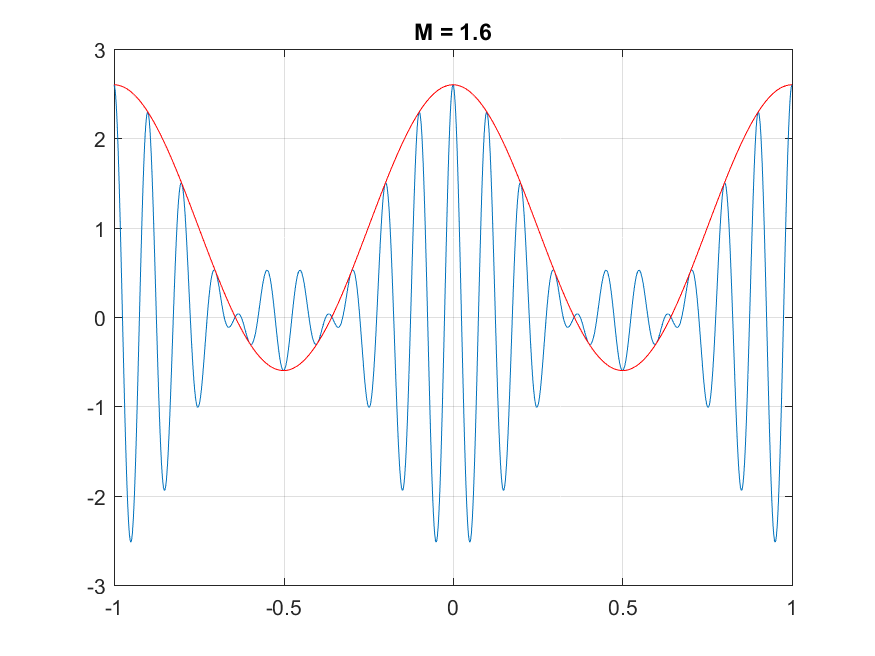
\includegraphics[scale=0.7]{sigm16.png}
		\caption{Результат АМ для m = 1.6} 
		\label{pic:pic01} % название для ссылок внутри кода
	\end{center}
\end{figure} 

\begin{figure}[H]
	\begin{center}
		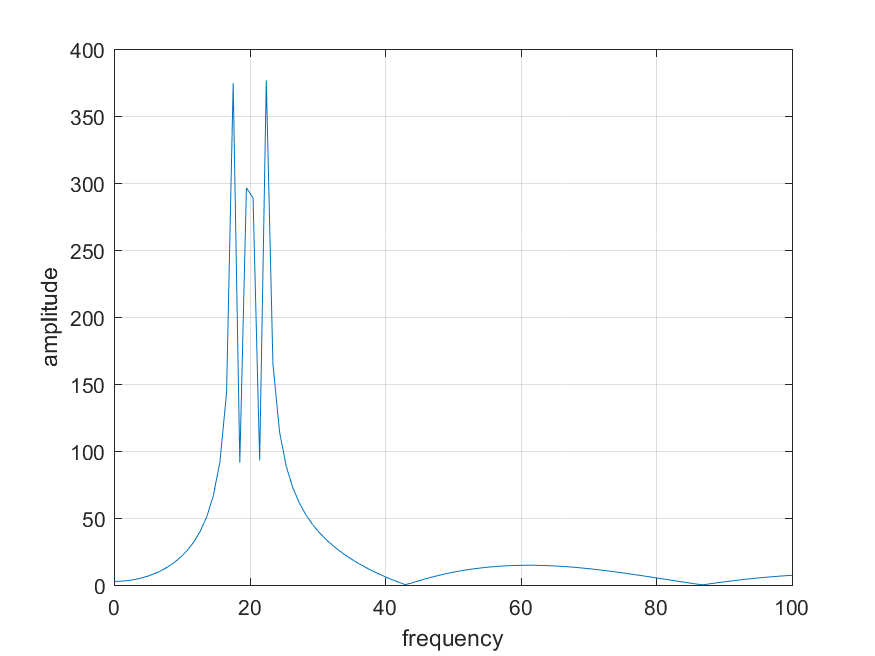
\includegraphics[scale=0.7]{specm16.png}
		\caption{Амплитудный спектр для m = 1.6} 
		\label{pic:pic02} % название для ссылок внутри кода
	\end{center}
\end{figure}
%%%%%%%%%%%%%%%%%%%%%%%%%%%%%%%%%%%%%%%%%%%%%%%%%%%%%%%%%%%
  

\begin{figure}[H]
	\begin{center}
		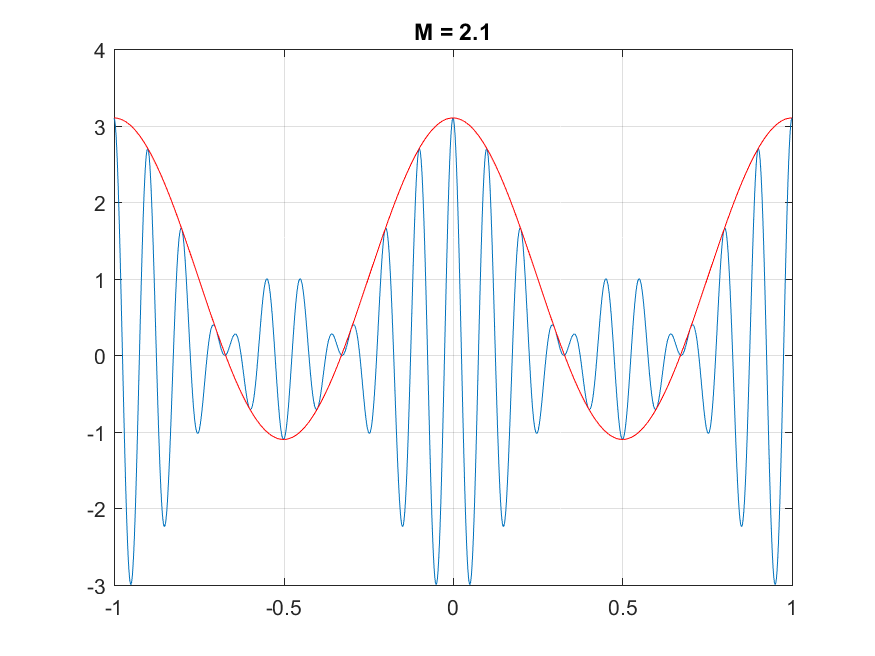
\includegraphics[scale=0.7]{sigm21.png}
		\caption{Результат АМ для m = 2.1} 
		\label{pic:pic01} % название для ссылок внутри кода
	\end{center}
\end{figure} 

\begin{figure}[H]
	\begin{center}
		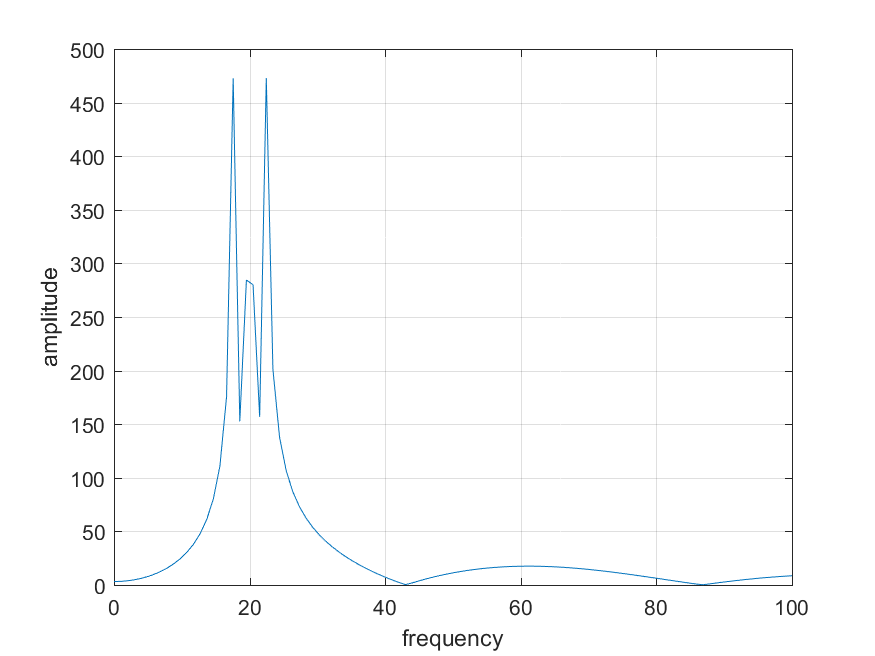
\includegraphics[scale=0.7]{specm21.png}
		\caption{Амплитудный спектр для m = 2.1} 
		\label{pic:pic02} % название для ссылок внутри кода
	\end{center}
\end{figure}
%%%%%%%%%%%%%%%%%%%%%%%%%%%%%%%%%%%%%%%%%%%%%%%%%%%%%%%%%%%
\begin{figure}[H]
	\begin{center}
		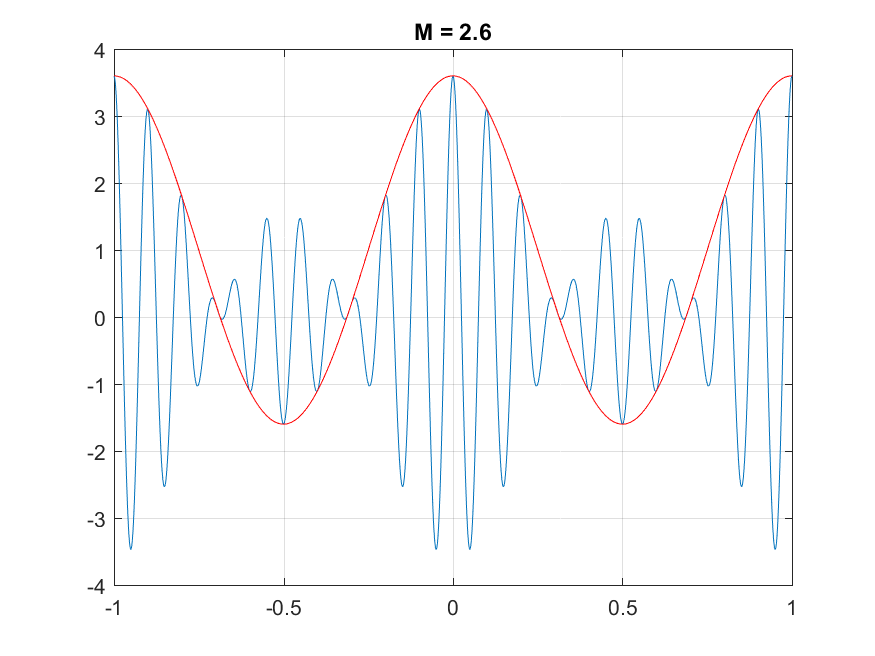
\includegraphics[scale=0.7]{sigm26.png}
		\caption{Результат АМ для m = 2.6} 
		\label{pic:pic01} % название для ссылок внутри кода
	\end{center}
\end{figure} 

\begin{figure}[H]
	\begin{center}
		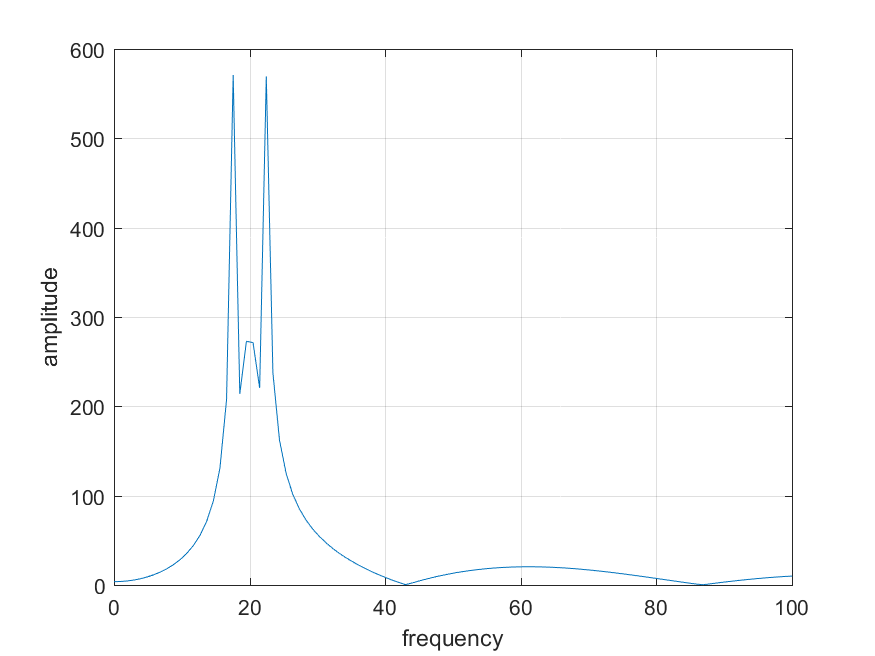
\includegraphics[scale=0.7]{specm26.png}
		\caption{Амплитудный спектр для m = 2.6} 
		\label{pic:pic02} % название для ссылок внутри кода
	\end{center}
\end{figure} 
%%%%%%%%%%%%%%%%%%%%%%%%%%%%%%%%%%%%%%%%%%%%%%%%%%%%%%%%
В ходе проведения данной части работы, мы экспериментально подтвердили, что коэффициент модуляции
является важным параметром модуляции сигнала. Также путем эксперимента выяснили,
что наилучшее качество модуляции получается при $ 0.5 < m < 1 $. 
\subsection{КПД АМ для однотонального канала}
Также мы рассчитаем КПД амплитудной модуляции 

\begin{figure}[H]
	\begin{center}
		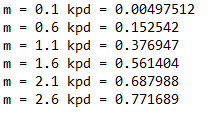
\includegraphics[scale=0.7]{kpd.png}
		\caption{Расчет КПД} 
		\label{pic:pic02} % название для ссылок внутри кода
	\end{center}
\end{figure} 

Проанализировав полученные значения, можно сделать вывод, что КПД при самых эффективных значениях коэффициента m
находится в промежутке $ 0.15 < \nu < 0.37 $. Теория подтверждает, что обычная амплитудная модуляция
имеет очень низкий коэффициент полезного действия.

   
\subsection{Модуляция с подавлением несущей}
Далее проведем модуляцию c подавлением несущей.
Проделаем это также с помощью функций встроенного пакета Communications в Matlab.
	
%%%%%%%%%%%%%%%%%%%%%%%%%%%%%%%%%%%%%%%%%%%%%%%%%%%%%%%%%%%
\begin{figure}[H]
	\begin{center}
		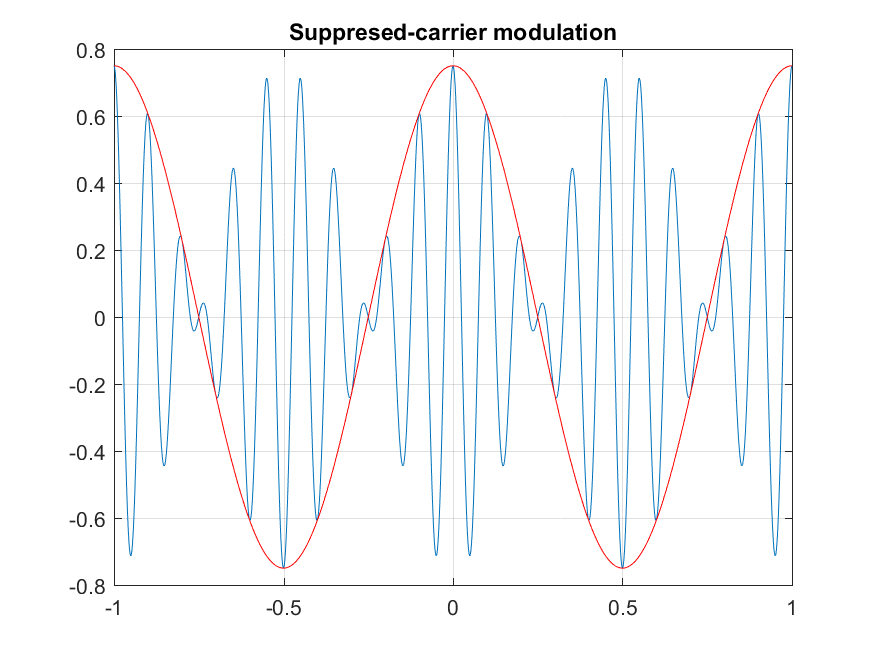
\includegraphics[scale=0.7]{supcar.png}
		\caption{Модулированный сигнал с подавлением несущей} 
		\label{pic:pic01} % название для ссылок внутри кода
	\end{center}
\end{figure} 
Также построим спектр модулированного сигнала.
\begin{figure}[H]
	\begin{center}
		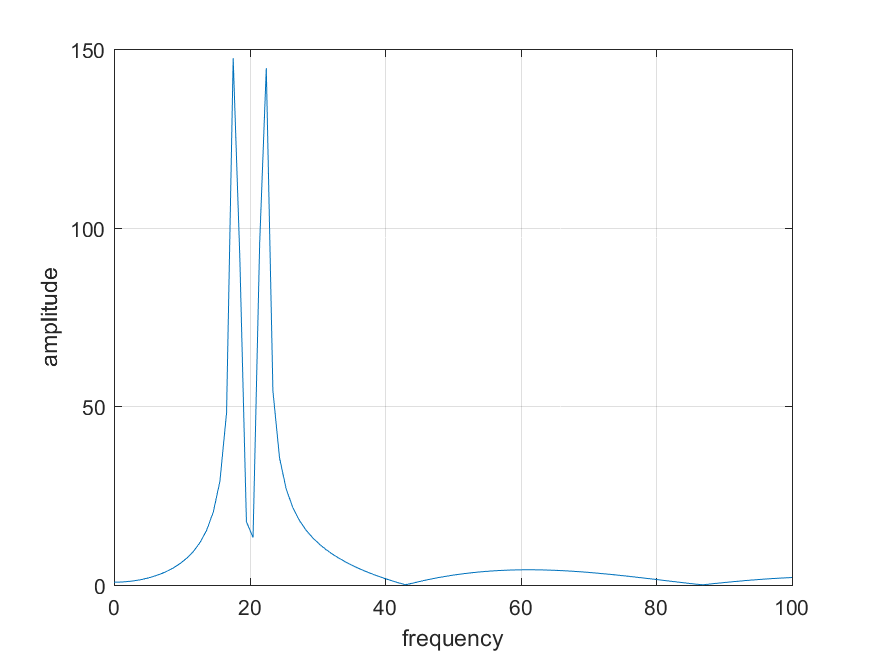
\includegraphics[scale=0.7]{specsupcar.png}
		\caption{Амплитудный спектр} 
		\label{pic:pic02} % название для ссылок внутри кода
	\end{center}
\end{figure} 
Из графика спектра становится понятно, почему модуляция с подавлением несущей.
Также следует отметить, что за счет подавления несущей мы повышаем КПД.  
%%%%%%%%%%%%%%%%%%%%%%%%%%%%%%%%%%%%%%%%%%%%%%%%%%%%%%%%

\subsection{Однополосная модуляция}
Далее проведем однополосную модуляцию в соответствии с теорией.
Получим модулируемый сигнал.
\begin{figure}[H]
	\begin{center}
		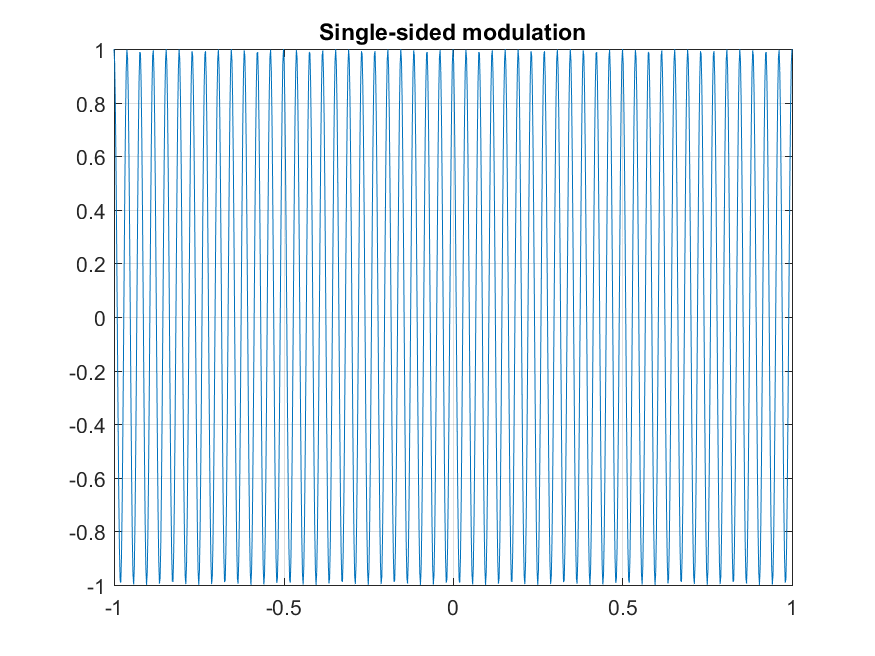
\includegraphics[scale=0.7]{singside.png}
		\caption{Однополосная модуляция} 
		\label{pic:pic02} % название для ссылок внутри кода
	\end{center}
\end{figure} 
Далее вручную реализуем алгоритм демодуляции:

\begin{itemize}
	\item домножаем на опорное колебание 
	\item проводим фильтрацию с помощью низкочастотного фильтра, в нашем случае Баттерворта 
	\item получаем искомый информационный сигнал.
\end{itemize}
В результате получаем, почти полное совпадение демодулированного сигнала(синий) с моделирующим(красный).
\begin{figure}[H]
	\begin{center}
		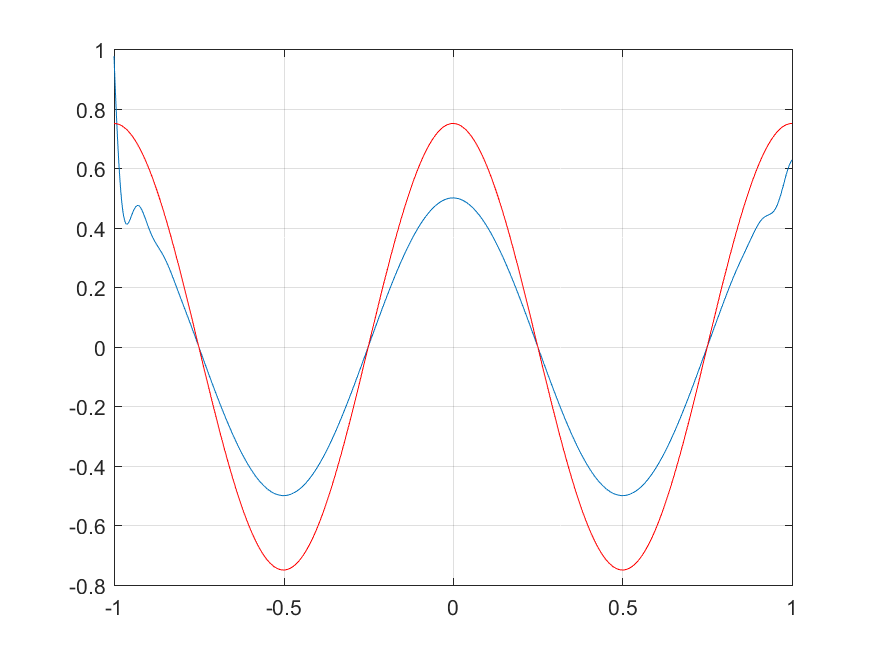
\includegraphics[scale=0.7]{singsideres.png}
		\caption{Амплитудный спектр} 
		\label{pic:pic02} % название для ссылок внутри кода
	\end{center}
\end{figure}    

\section{Выводы}
В ходе проделанной работы мы познакомились с одним из типов аналоговй модуляцией - амплитудной.
Нам удалось разобраться в алгоритмах модуляции и демодуляции, и даже самим реализовать их в Matlab с помощью пакета Communications. Также мы узнали о различных типах аналоговой модуляции:
\begin{itemize}
	\item обычная амплитудная модуляция(amplitude modulation)
	\item амплитудная модуляция с подавлением несущей (suppresed-carrier modulation)
	\item однополосная модуляция(single side band modulation).
\end{itemize}
Нам удалось на качественном уровне разобраться с процессом работы каждого из типов.
Также мы смогли вычислить КПД обычной модуляции на примере модуляции однотонального сигнала.
В результате чего, мы экспериментально подтвердили, что значения КПД при данном виде модуляции достаточно низки. 

\end{document}
